% Options for packages loaded elsewhere
\PassOptionsToPackage{unicode}{hyperref}
\PassOptionsToPackage{hyphens}{url}
\PassOptionsToPackage{dvipsnames,svgnames,x11names}{xcolor}
%
\documentclass[
  letterpaper,
  DIV=11,
  numbers=noendperiod]{scrartcl}

\usepackage{amsmath,amssymb}
\usepackage{iftex}
\ifPDFTeX
  \usepackage[T1]{fontenc}
  \usepackage[utf8]{inputenc}
  \usepackage{textcomp} % provide euro and other symbols
\else % if luatex or xetex
  \usepackage{unicode-math}
  \defaultfontfeatures{Scale=MatchLowercase}
  \defaultfontfeatures[\rmfamily]{Ligatures=TeX,Scale=1}
\fi
\usepackage{lmodern}
\ifPDFTeX\else  
    % xetex/luatex font selection
\fi
% Use upquote if available, for straight quotes in verbatim environments
\IfFileExists{upquote.sty}{\usepackage{upquote}}{}
\IfFileExists{microtype.sty}{% use microtype if available
  \usepackage[]{microtype}
  \UseMicrotypeSet[protrusion]{basicmath} % disable protrusion for tt fonts
}{}
\makeatletter
\@ifundefined{KOMAClassName}{% if non-KOMA class
  \IfFileExists{parskip.sty}{%
    \usepackage{parskip}
  }{% else
    \setlength{\parindent}{0pt}
    \setlength{\parskip}{6pt plus 2pt minus 1pt}}
}{% if KOMA class
  \KOMAoptions{parskip=half}}
\makeatother
\usepackage{xcolor}
\setlength{\emergencystretch}{3em} % prevent overfull lines
\setcounter{secnumdepth}{-\maxdimen} % remove section numbering
% Make \paragraph and \subparagraph free-standing
\makeatletter
\ifx\paragraph\undefined\else
  \let\oldparagraph\paragraph
  \renewcommand{\paragraph}{
    \@ifstar
      \xxxParagraphStar
      \xxxParagraphNoStar
  }
  \newcommand{\xxxParagraphStar}[1]{\oldparagraph*{#1}\mbox{}}
  \newcommand{\xxxParagraphNoStar}[1]{\oldparagraph{#1}\mbox{}}
\fi
\ifx\subparagraph\undefined\else
  \let\oldsubparagraph\subparagraph
  \renewcommand{\subparagraph}{
    \@ifstar
      \xxxSubParagraphStar
      \xxxSubParagraphNoStar
  }
  \newcommand{\xxxSubParagraphStar}[1]{\oldsubparagraph*{#1}\mbox{}}
  \newcommand{\xxxSubParagraphNoStar}[1]{\oldsubparagraph{#1}\mbox{}}
\fi
\makeatother


\providecommand{\tightlist}{%
  \setlength{\itemsep}{0pt}\setlength{\parskip}{0pt}}\usepackage{longtable,booktabs,array}
\usepackage{calc} % for calculating minipage widths
% Correct order of tables after \paragraph or \subparagraph
\usepackage{etoolbox}
\makeatletter
\patchcmd\longtable{\par}{\if@noskipsec\mbox{}\fi\par}{}{}
\makeatother
% Allow footnotes in longtable head/foot
\IfFileExists{footnotehyper.sty}{\usepackage{footnotehyper}}{\usepackage{footnote}}
\makesavenoteenv{longtable}
\usepackage{graphicx}
\makeatletter
\def\maxwidth{\ifdim\Gin@nat@width>\linewidth\linewidth\else\Gin@nat@width\fi}
\def\maxheight{\ifdim\Gin@nat@height>\textheight\textheight\else\Gin@nat@height\fi}
\makeatother
% Scale images if necessary, so that they will not overflow the page
% margins by default, and it is still possible to overwrite the defaults
% using explicit options in \includegraphics[width, height, ...]{}
\setkeys{Gin}{width=\maxwidth,height=\maxheight,keepaspectratio}
% Set default figure placement to htbp
\makeatletter
\def\fps@figure{htbp}
\makeatother

\KOMAoption{captions}{tableheading}
\makeatletter
\@ifpackageloaded{caption}{}{\usepackage{caption}}
\AtBeginDocument{%
\ifdefined\contentsname
  \renewcommand*\contentsname{Table of contents}
\else
  \newcommand\contentsname{Table of contents}
\fi
\ifdefined\listfigurename
  \renewcommand*\listfigurename{List of Figures}
\else
  \newcommand\listfigurename{List of Figures}
\fi
\ifdefined\listtablename
  \renewcommand*\listtablename{List of Tables}
\else
  \newcommand\listtablename{List of Tables}
\fi
\ifdefined\figurename
  \renewcommand*\figurename{Figure}
\else
  \newcommand\figurename{Figure}
\fi
\ifdefined\tablename
  \renewcommand*\tablename{Table}
\else
  \newcommand\tablename{Table}
\fi
}
\@ifpackageloaded{float}{}{\usepackage{float}}
\floatstyle{ruled}
\@ifundefined{c@chapter}{\newfloat{codelisting}{h}{lop}}{\newfloat{codelisting}{h}{lop}[chapter]}
\floatname{codelisting}{Listing}
\newcommand*\listoflistings{\listof{codelisting}{List of Listings}}
\makeatother
\makeatletter
\makeatother
\makeatletter
\@ifpackageloaded{caption}{}{\usepackage{caption}}
\@ifpackageloaded{subcaption}{}{\usepackage{subcaption}}
\makeatother

\ifLuaTeX
  \usepackage{selnolig}  % disable illegal ligatures
\fi
\usepackage{bookmark}

\IfFileExists{xurl.sty}{\usepackage{xurl}}{} % add URL line breaks if available
\urlstyle{same} % disable monospaced font for URLs
\hypersetup{
  pdftitle={Administración del Efectivo},
  pdfauthor={Docente: Carlos Correa Iñiguez (ca.correai@profesor.duoc.cl)},
  colorlinks=true,
  linkcolor={blue},
  filecolor={Maroon},
  citecolor={Blue},
  urlcolor={Blue},
  pdfcreator={LaTeX via pandoc}}


\title{Administración del Efectivo}
\author{Docente: Carlos Correa Iñiguez
(\href{mailto:ca.correai@profesor.duoc.cl}{\nolinkurl{ca.correai@profesor.duoc.cl}})}
\date{}

\begin{document}
\maketitle


\subsubsection{Objetivos de la Clase:}\label{objetivos-de-la-clase}

1. \textbf{Conocer los principales modelos de administración del
efectivo}, entendiendo su importancia en la gestión financiera
empresarial. 2. \textbf{Aplicar los componentes clave de cada modelo},
asegurando una gestión eficiente y óptima del efectivo en la
organización.

\begin{center}\rule{0.5\linewidth}{0.5pt}\end{center}

\subsubsection{Administración de la
liquidez}\label{administraciuxf3n-de-la-liquidez}

\begin{figure}[H]

{\centering 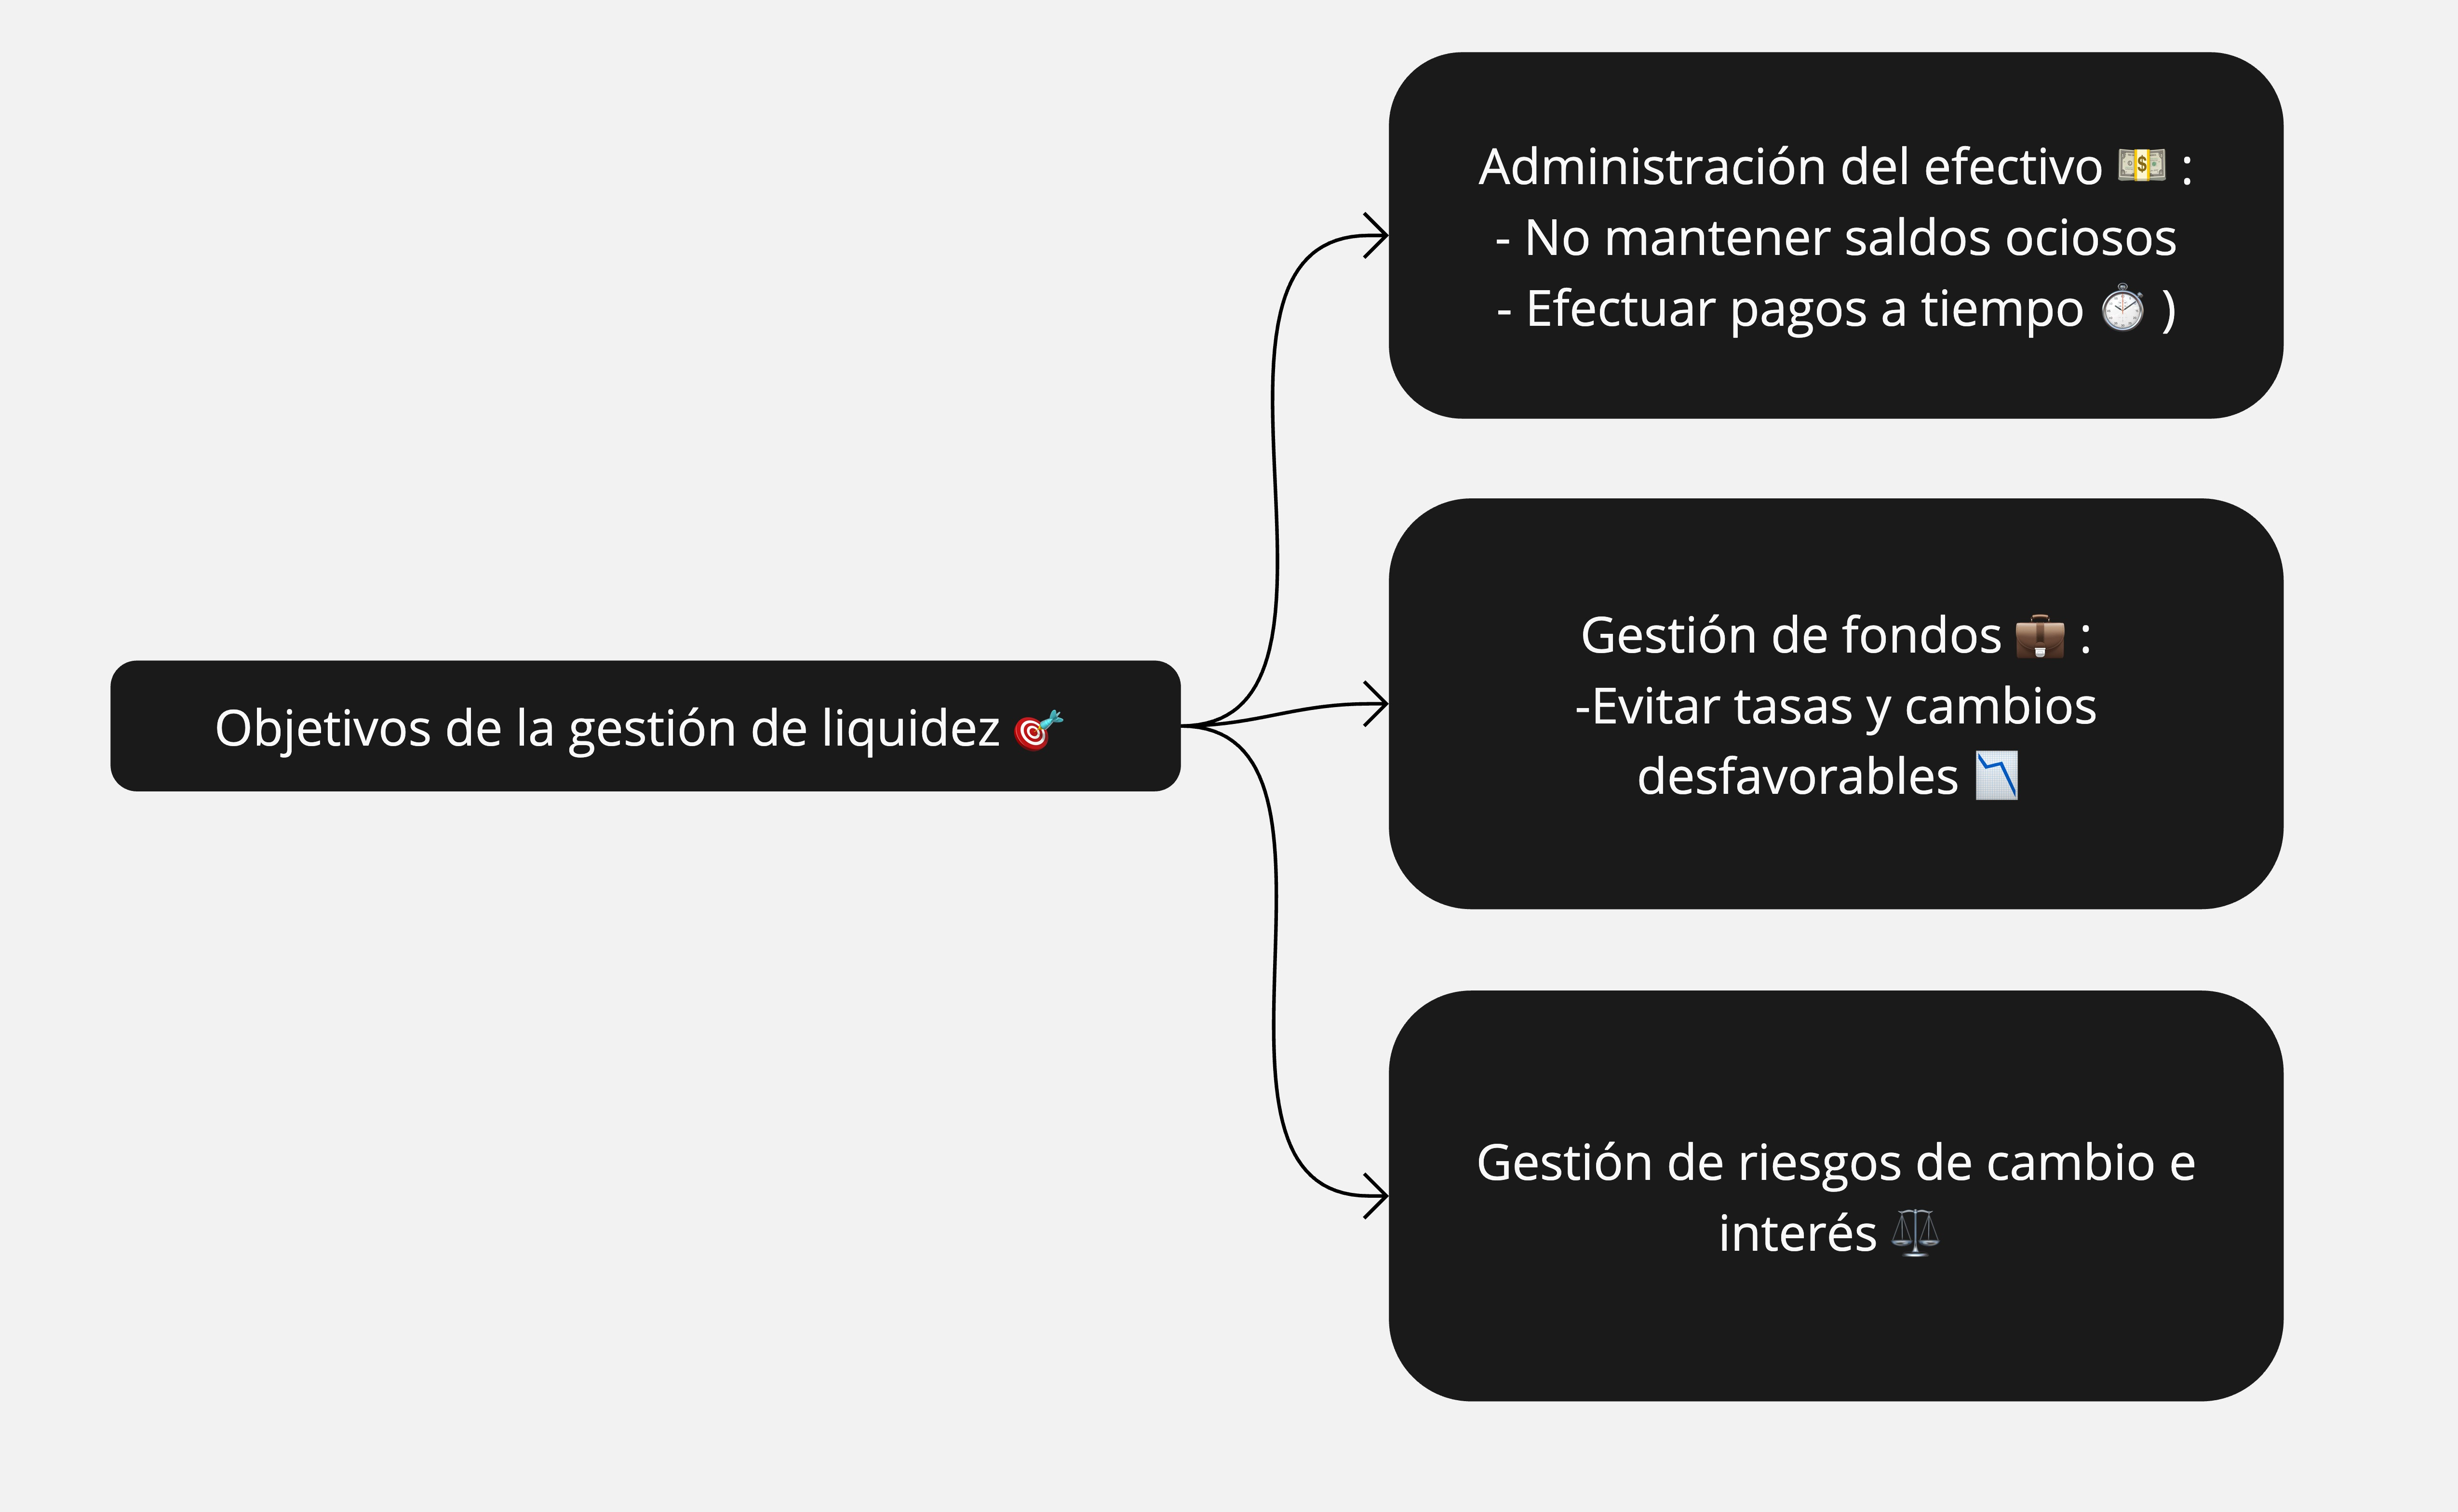
\includegraphics{Imagen2.png}

}

\caption{Administración de la liquidez}

\end{figure}%

\begin{center}\rule{0.5\linewidth}{0.5pt}\end{center}

\subsubsection{Administración de Efectivo
(Brealey)}\label{administraciuxf3n-de-efectivo-brealey}

Según Brealey, el efectivo se define a menudo como \textbf{``un activo
que no genera utilidades''}.

\begin{itemize}
\tightlist
\item
  Su tenencia es necesaria para pagar mano de obra, materia prima,
  impuestos, dividendos, y comprar activos fijos.
\item
  Aunque el efectivo no genera intereses, la tarea del administrador
  financiero es \textbf{minimizar} la cantidad de efectivo manteniendo
  suficiente liquidez para:

  \begin{itemize}
  \tightlist
  \item
    Aprovechar descuentos comerciales
  \item
    Mantener la reputación crediticia
  \item
    Satisfacer necesidades imprevistas
  \end{itemize}
\end{itemize}

\begin{center}\rule{0.5\linewidth}{0.5pt}\end{center}

\subsection{Administración del Efectivo
(Gitman)}\label{administraciuxf3n-del-efectivo-gitman}

\begin{itemize}
\tightlist
\item
  Es un activo clave en la \textbf{gestión del capital de trabajo}.
\item
  Permite pagar facturas a tiempo y funciona como un \textbf{colchón
  financiero} para imprevistos.
\item
  Los activos circulantes, como cuentas por cobrar e inventarios, se
  convierten en efectivo, el \textbf{denominador común} de los activos
  líquidos.
\end{itemize}

\begin{center}\rule{0.5\linewidth}{0.5pt}\end{center}

\subsection{Estrategias de Administración de
Efectivo}\label{estrategias-de-administraciuxf3n-de-efectivo}

Según Gitman, las principales estrategias son:

\begin{enumerate}
\def\labelenumi{\arabic{enumi}.}
\tightlist
\item
  \textbf{Cuentas por pagar}: Pagar lo más tarde posible sin afectar la
  reputación crediticia, aprovechando descuentos por pronto pago.
\item
  \textbf{Inventario}: Rotar el inventario rápidamente para evitar
  agotamientos que afecten la producción o las ventas.
\item
  \textbf{Cuentas por cobrar}: Cobrar lo más rápido posible sin
  presionar a los clientes, utilizando descuentos por pago de contado
  cuando sea económicamente viable.
\end{enumerate}

\begin{center}\rule{0.5\linewidth}{0.5pt}\end{center}

\subsubsection{Objetvos de la administración del
efectivo:}\label{objetvos-de-la-administraciuxf3n-del-efectivo}

El principal objetivo de la administración del efectivo es
\textbf{minimizar la inversión en efectivo} sin comprometer la
eficiencia operativa de la empresa. - \textbf{Saldo mínimo de efectivo}:
Determinar la cantidad mínima de efectivo que debe mantener la empresa,
considerando sus necesidades específicas y características operativas. -
\textbf{Ciclo de caja}: Definir el número de días que transcurren desde
que la empresa realiza pagos a sus proveedores hasta que recibe los
cobros de sus clientes, asegurando una gestión óptima del flujo de
efectivo.

\begin{center}\rule{0.5\linewidth}{0.5pt}\end{center}

\begin{figure}[H]

{\centering 
\includegraphics{Imagen1.png}

}

\caption{Ciclo Operativo}

\end{figure}%

\begin{center}\rule{0.5\linewidth}{0.5pt}\end{center}

\subsubsection{Modelos de Administración del
Efectivo}\label{modelos-de-administraciuxf3n-del-efectivo}

\begin{enumerate}
\def\labelenumi{\arabic{enumi}.}
\tightlist
\item
  \textbf{Modelo de Pérdida Operativa Mínima (POM)}: Minimiza los costos
  del mantenimiento de efectivo, asegurando suficiente liquidez para las
  operaciones.
\item
  \textbf{Modelo de Baumol}: Calcula el saldo óptimo de efectivo basado
  en los costos de transacción y el costo de oportunidad.
\item
  \textbf{Modelo de Miller y Orr}: Controla los saldos de efectivo
  estableciendo límites superior e inferior, ajustando automáticamente
  según las fluctuaciones.
\end{enumerate}

\begin{center}\rule{0.5\linewidth}{0.5pt}\end{center}

\subsubsection{Modelo de Pérdida Operativa Mínima
(POM)}\label{modelo-de-puxe9rdida-operativa-muxednima-pom}

\begin{itemize}
\tightlist
\item
  \textbf{Objetivo}: Minimizar los costos de mantener efectivo sin
  comprometer la operación.
\item
  \textbf{Principio}: Determina el saldo mínimo de efectivo que la
  empresa debe mantener para operar eficientemente.
\item
  \textbf{Ventaja}: Optimiza la liquidez, reduciendo el costo de
  oportunidad de mantener grandes cantidades de efectivo sin invertir.
\end{itemize}

\begin{center}\rule{0.5\linewidth}{0.5pt}\end{center}

\subsubsection{Fórmulas del Modelo
POM}\label{fuxf3rmulas-del-modelo-pom}

\paragraph{\texorpdfstring{1. \textbf{Rotación de
Caja}:}{1. Rotación de Caja:}}\label{rotaciuxf3n-de-caja}

\[
   R_c = \frac{\text{360}}{\text{Ciclo de Caja}}
   \] - \(R_c\): Rotación de caja, mide cuántas veces la empresa
``gira'' su efectivo durante el año.

\subsubsection{\texorpdfstring{2. \textbf{Caja
Mínima}:}{2. Caja Mínima:}}\label{caja-muxednima}

\[
   C_{\text{mínima}} = \frac{\text{Desembolsos Anuales}}{\text{Rotación de Caja}}
   \] - \textbf{C\_\{\text{mínima}\}}: Cantidad mínima de efectivo que
la empresa debe mantener para operar.

\subsubsection{Fórmula del POM (Pérdida Operativa
Mínima):}\label{fuxf3rmula-del-pom-puxe9rdida-operativa-muxednima}

\[
   \text{POM} = C_{\text{mínima}} + \text{Costos de Oportunidad}
   \] - \textbf{POM}: Es la pérdida que incurre la empresa por mantener
el saldo mínimo de caja, sumando el costo de oportunidad de no invertir
ese efectivo.

\begin{center}\rule{0.5\linewidth}{0.5pt}\end{center}

\subsubsection{Ejemplo (POM)}\label{ejemplo-pom}

Indicadores de gestión:

\begin{itemize}
\tightlist
\item
  \textbf{Período promedio de cobro}: 60 días
\item
  \textbf{Período promedio de pago}: 45 días
\item
  \textbf{Período promedio de inventario}: 75 días
\item
  \textbf{Desembolsos anuales}: \$10.000.000
\item
  \textbf{Costo de oportunidad}: 18\%
\end{itemize}

\begin{center}\rule{0.5\linewidth}{0.5pt}\end{center}

\subsubsection{Solucion Parte I:}\label{solucion-parte-i}

\paragraph{Cálculos del Ciclo de Caja y
POM}\label{cuxe1lculos-del-ciclo-de-caja-y-pom}

\begin{enumerate}
\def\labelenumi{\arabic{enumi}.}
\tightlist
\item
  \textbf{Ciclo Operativo}: \[
  \text{Ciclo Operativo} = PPI + PPC
  \] \[
  \text{Ciclo Operativo} = 75 + 60 = 135 \, \text{días}
  \] Donde:

  \begin{itemize}
  \tightlist
  \item
    \(PPI\): Período Promedio de Inventario
  \item
    \(PPC\): Período Promedio de Cobro
  \end{itemize}
\end{enumerate}

\begin{center}\rule{0.5\linewidth}{0.5pt}\end{center}

\subsubsection{Solucion Parte II:}\label{solucion-parte-ii}

\begin{enumerate}
\def\labelenumi{\arabic{enumi}.}
\setcounter{enumi}{1}
\tightlist
\item
  \textbf{Ciclo de Efectivo}: \[
   \text{Ciclo de Efectivo} = \text{Ciclo Operativo} - PPP
   \] \[
   \text{Ciclo de Efectivo} = 135 - 45 = 90 \, \text{días}
   \] Donde:

  \begin{itemize}
  \tightlist
  \item
    \(PPP\): Período Promedio de Pago
  \end{itemize}
\end{enumerate}

\begin{center}\rule{0.5\linewidth}{0.5pt}\end{center}

\subsubsection{Solucion Solucion Parte
III}\label{solucion-solucion-parte-iii}

\paragraph{Cálculos del Ciclo de Caja y
POM}\label{cuxe1lculos-del-ciclo-de-caja-y-pom-1}

\begin{enumerate}
\def\labelenumi{\arabic{enumi}.}
\setcounter{enumi}{2}
\item
  \textbf{Rotación de Caja}: \[
  \text{Rotación de Caja} = \frac{360}{\text{Ciclo de Efectivo}} = \frac{360}{90} = 4 \, \text{veces}
  \]
\item
  \textbf{Caja Mínima}: \[
  \text{Caja Mínima} = \frac{\text{Desembolsos Anuales}}{\text{Rotación de Caja}} = \frac{10.000.000}{4} = 2.500.000
  \]
\item
  \textbf{Pérdida Operativa Mínima (POM)}: \[
  \text{POM} = \text{Caja Mínima} \times k_o = 2.500.000 \times 18\% = 450.000
  \] Donde:

  \begin{itemize}
  \tightlist
  \item
    \(k_o\): Costo de Oportunidad.
  \end{itemize}
\end{enumerate}

\begin{center}\rule{0.5\linewidth}{0.5pt}\end{center}

\subsubsection{Ciclo Operativo Ejemplo}\label{ciclo-operativo-ejemplo}

\begin{figure}[H]

{\centering 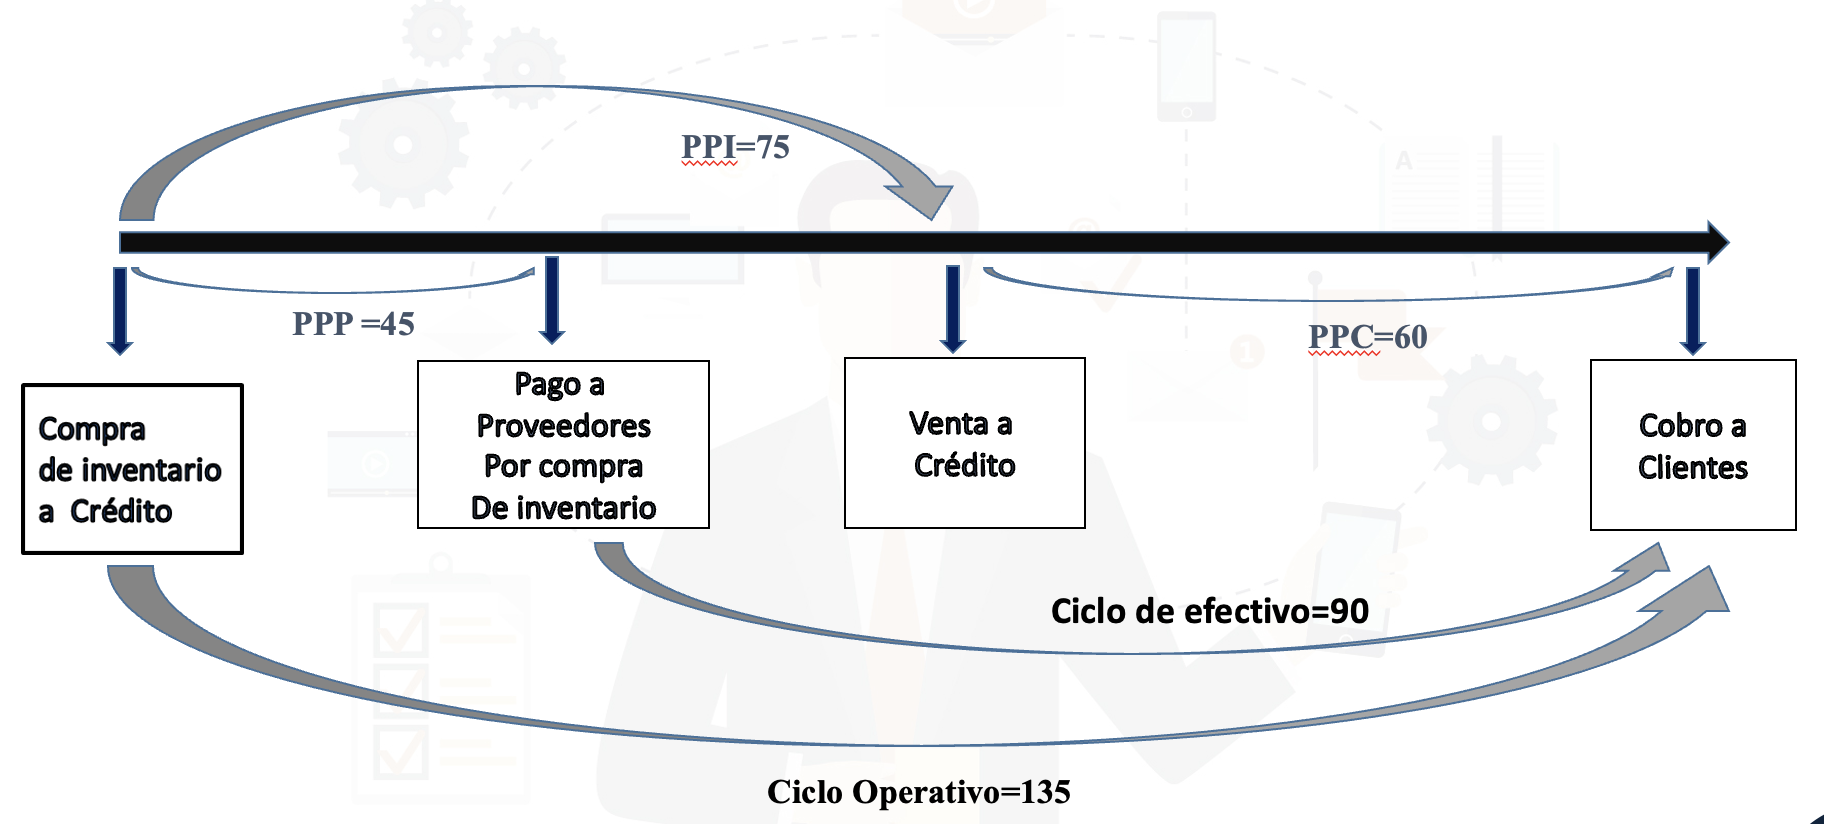
\includegraphics{Imagen4.png}

}

\caption{Ciclo Operativo Ejemplo}

\end{figure}%

\begin{center}\rule{0.5\linewidth}{0.5pt}\end{center}

\subsection{Interpretación de Resultados
I}\label{interpretaciuxf3n-de-resultados-i}

\begin{itemize}
\tightlist
\item
  \textbf{Ciclo Operativo}: La empresa tiene un ciclo operativo de
  \textbf{135 días}, que cubre el tiempo desde la compra de materias
  primas hasta el cobro de las ventas:

  \begin{enumerate}
  \def\labelenumi{\arabic{enumi}.}
  \tightlist
  \item
    Compra de mercaderías o materias primas.
  \item
    Producción y obtención de productos terminados.
  \item
    Venta de los productos.
  \item
    Cobro a clientes (generación del flujo de caja).
  \end{enumerate}
\end{itemize}

\begin{center}\rule{0.5\linewidth}{0.5pt}\end{center}

\subsection{Interpretación de Resultados
II}\label{interpretaciuxf3n-de-resultados-ii}

\begin{itemize}
\tightlist
\item
  \textbf{Ciclo de Efectivo}: El ciclo de efectivo es de \textbf{90
  días}, debido a un período de financiación de \textbf{45 días}
  otorgado por los proveedores.
\item
  \textbf{Rotación de Caja}: La empresa rota su efectivo \textbf{4 veces
  al año}. Una mayor rotación significa que se requiere menos efectivo
  disponible para operar eficientemente.
\end{itemize}

\begin{center}\rule{0.5\linewidth}{0.5pt}\end{center}

\subsubsection{Modelo de W. Baumol}\label{modelo-de-w.-baumol}

\begin{itemize}
\tightlist
\item
  \textbf{Objetivo}: Minimizar costos de transacción y mantener un saldo
  óptimo de efectivo.
\item
  \textbf{Principio}: Equilibra el costo de mantener efectivo y
  convertir activos.
\item
  \textbf{Ventaja}: Ideal para empresas con flujos constantes,
  reduciendo la frecuencia de transacciones.
\end{itemize}

\begin{center}\rule{0.5\linewidth}{0.5pt}\end{center}

\subsubsection{Formula de Modelo de W.
Baumol}\label{formula-de-modelo-de-w.-baumol}

\[ 
C = \sqrt{\frac{2 \cdot T \cdot b}{i}}
\] - \(C\): Saldo óptimo de efectivo. - \(T\): Necesidades de efectivo
al año. - \(b\): Costo de convertir valores negociables. - \(i\): Tasa
de interés.

\begin{center}\rule{0.5\linewidth}{0.5pt}\end{center}

\subsection{Modelo de Baumol}\label{modelo-de-baumol}

El modelo de Baumol identifica dos costos principales: 1. \textbf{Costo
de Transacción}: Representa el costo por ordenamiento o comercial. 2.
\textbf{Costo de Oportunidad}: Representa el costo de mantener efectivo
disponible. - \textbf{Costo Total}: La suma de ambos costos corresponde
al costo total del efectivo: \[
\text{Costo Total} = \text{Costo de Transacción} + \text{Costo de Oportunidad} 
\]

\begin{center}\rule{0.5\linewidth}{0.5pt}\end{center}

\subsection{Costo de Transacción (b)}\label{costo-de-transacciuxf3n-b}

- \textbf{Costo de Transacción (b)}: Es el costo de convertir valores
negociables a efectivo. Este costo es constante y está influido por el
número de transacciones realizadas, e incluye costos de oficina y
transacción. - \textbf{Número de Transacciones}: Se calcula como:

\[ 
  \text{Número de Transacciones} = \frac{t}{c} 
  \]

Donde:

\begin{itemize}
\tightlist
\item
  t: Necesidades de efectivo al año.
\item
  c: Saldo de efectivo óptimo.
\end{itemize}

\begin{center}\rule{0.5\linewidth}{0.5pt}\end{center}

\subsubsection{Costo por Ordenamiento}\label{costo-por-ordenamiento}

\begin{itemize}
\tightlist
\item
  El costo por ordenamiento se calcula como: \[
    \text{Costo por Ordenamiento} = b \times \left( \frac{t}{c} \right)
    \] Donde \(b\) es el costo de cada transacción multiplicado por el
  número de transacciones necesarias en el periodo.

  \begin{itemize}
  \tightlist
  \item
    t: Necesidades de efectivo al año.
  \item
    c: Saldo de efectivo óptimo.
  \end{itemize}
\end{itemize}

\begin{center}\rule{0.5\linewidth}{0.5pt}\end{center}

\subsection{Costo de Oportunidad (i)}\label{costo-de-oportunidad-i}

\begin{itemize}
\tightlist
\item
  \textbf{Costo de Oportunidad (i)}: Se determina por la tasa de interés
  no aprovechada, que podría haberse obtenido al invertir el saldo de
  efectivo \(c\) en el mercado financiero.
\end{itemize}

- Según el modelo de Baumol, los \textbf{saldos de efectivo} siguen un
patrón constante, comenzando con un saldo \(c\) al inicio del periodo y
disminuyendo gradualmente hasta cero.

\begin{itemize}
\item
  El saldo medio de efectivo se representa como:

  \[ 
  \text{Saldos Medios de Efectivo} = \frac{c}{2}
  \]
\end{itemize}

\begin{center}\rule{0.5\linewidth}{0.5pt}\end{center}

\subsubsection{Costo de Mantenimiento de
Efectivo}\label{costo-de-mantenimiento-de-efectivo}

\begin{itemize}
\item
  El costo de oportunidad \(i\), multiplicado por los saldos medios de
  efectivo, da como resultado el \textbf{costo de mantenimiento}:

  \[ 
  \text{Costo de Mantenimiento} = i \times \left( \frac{c}{2} \right)
  \]
\end{itemize}

\begin{center}\rule{0.5\linewidth}{0.5pt}\end{center}

\subsection{Costo Total de Efectivo}\label{costo-total-de-efectivo}

\begin{itemize}
\item
  La suma del costo de mantenimiento y el costo de ordenamiento nos da
  el \textbf{Costo Total de Efectivo}:

  \[ 
  \text{Costo Total} = b \times \left( \frac{t}{c} \right) + i \times \left( \frac{c}{2} \right)
  \]
\item
  A medida que \textbf{c} aumenta:

  \begin{itemize}
  \tightlist
  \item
    El \textbf{Costo de Oportunidad} (\(i \times \frac{c}{2}\)) aumenta.
  \item
    El \textbf{Costo Comercial} (\(b \times \frac{t}{c}\)) disminuye.
  \end{itemize}
\end{itemize}

\subsubsection{Equilibrio de Costos}\label{equilibrio-de-costos}

\begin{itemize}
\item
  La cantidad óptima de efectivo se obtiene cuando el \textbf{Costo de
  Oportunidad} es igual al \textbf{Costo Comercial}:

  \[ 
  b \times \left( \frac{t}{c} \right) = i \times \left( \frac{c}{2} \right)
  \]
\end{itemize}

\begin{center}\rule{0.5\linewidth}{0.5pt}\end{center}

\subsubsection{Ejemplo (Baumol)}\label{ejemplo-baumol}

Una empresa realiza sus compras de mercadería a 30 días (periodo de
financiación de proveedor), el periodo de inventarios es de 45 días y el
periodo de cuentas por cobrar es de 45 días. Para un periodo de 60 días
la empresa requiere \$80.000.000.Se ha estimado que para una venta de
valores negociables se incurrirá en un costo de \$80.000 por cada
transacción. La rentabilidad de los valores negociables se estima en
15\% anual.

\begin{center}\rule{0.5\linewidth}{0.5pt}\end{center}

\subsubsection{Se pide:}\label{se-pide}

\begin{itemize}
\tightlist
\item
  \begin{enumerate}
  \def\labelenumi{\alph{enumi})}
  \tightlist
  \item
    Determinar el ciclo operativo y el ciclo de efectivo
  \end{enumerate}
\item
  \begin{enumerate}
  \def\labelenumi{\alph{enumi})}
  \setcounter{enumi}{1}
  \tightlist
  \item
    Cantidad de dinero por transacción (Modelo de W. Baumol)
  \end{enumerate}
\item
  \begin{enumerate}
  \def\labelenumi{\alph{enumi})}
  \setcounter{enumi}{2}
  \tightlist
  \item
    Número de transacciones en 60 días
  \end{enumerate}
\item
  \begin{enumerate}
  \def\labelenumi{\alph{enumi})}
  \setcounter{enumi}{3}
  \tightlist
  \item
    Costo total aplicado al efectivo
  \end{enumerate}
\end{itemize}

\begin{center}\rule{0.5\linewidth}{0.5pt}\end{center}

\subsection{Ciclo Operativo y Ciclo de
Efectivo}\label{ciclo-operativo-y-ciclo-de-efectivo}

\begin{itemize}
\tightlist
\item
  \textbf{Ciclo Operativo}:
\end{itemize}

\[
Ciclo\ Operativo = \text{PPI} (45\ días) + \text{PPC} (45\ días) = 90\ días
\]

El Ciclo Operativo corresponde a 90 días, comenzando el día en que se
realizan las compras y terminando el día en que se realiza la cobranza
de las ventas.

\begin{center}\rule{0.5\linewidth}{0.5pt}\end{center}

\subsection{Ciclo de Efectivo}\label{ciclo-de-efectivo}

\begin{itemize}
\tightlist
\item
  \textbf{Ciclo de Efectivo}:
\end{itemize}

\[
Ciclo\ de\ Efectivo = (\text{PPI} - \text{PPP}) + \text{PPC}
\]

Sustituyendo los valores:

\[
Ciclo\ de\ Efectivo = (45 - 30) + 45 = 60\ días
\]

El ciclo de efectivo corresponde a 60 días, comenzando el día en que se
debe pagar a proveedores y terminando el día en que se realiza la
cobranza.

\begin{center}\rule{0.5\linewidth}{0.5pt}\end{center}

\subsection{Datos del Ejemplo}\label{datos-del-ejemplo}

\begin{itemize}
\tightlist
\item
  \(t = 80.000.000\) (Requerimiento de efectivo para un periodo de 60
  días)
\item
  \(b = 80.000\) (Costo de conversión de valores negociables)
\item
  \(n = 60\) días (Periodo de tiempo)
\item
  \(i = 15\%\) anual
\end{itemize}

\begin{center}\rule{0.5\linewidth}{0.5pt}\end{center}

\subsection{Cálculo de la Tasa
Bimestral}\label{cuxe1lculo-de-la-tasa-bimestral}

La tasa de costo de oportunidad bimestral se calcula como:

\[
i = \left(\frac{0.15}{360}\right) \times 60 = 0.025 = 2.5\%
\]

\subsubsection{Cálculo del Nivel Óptimo de
Efectivo}\label{cuxe1lculo-del-nivel-uxf3ptimo-de-efectivo}

El nivel óptimo de efectivo (\(C\)) se calcula utilizando la fórmula de
Baumol:

\[
C = \sqrt{\frac{2 \cdot b \cdot t}{i}}
\]

Sustituyendo los valores:

\[
C = \sqrt{\frac{2 \cdot 80.000 \cdot 80.000.000}{0.025}} = 22.627.417
\]

Este es el \textbf{nivel óptimo de efectivo}.

\begin{center}\rule{0.5\linewidth}{0.5pt}\end{center}

\subsection{Datos para el Cálculo}\label{datos-para-el-cuxe1lculo}

\begin{itemize}
\tightlist
\item
  \(t = \text{Necesidades de efectivo al año} = 80.000.000\)
\item
  \(b = \text{Costo de transacción} = 80.000\)
\end{itemize}

\subsubsection{Cálculo del Número de
Transacciones}\label{cuxe1lculo-del-nuxfamero-de-transacciones}

El número de transacciones se calcula como:

\[
\frac{t}{C} = \frac{80.000.000}{22.627.417} = 3.54
\]

\subsubsection{Cálculo del Costo
Comercial}\label{cuxe1lculo-del-costo-comercial}

El costo comercial se calcula como:

\[
\text{Costo Comercial} = b \times \frac{t}{C} = 80.000 \times \frac{80.000.000}{22.627.417} = 282.843
\]

Este es el \textbf{costo comercial} asociado al proceso.

\begin{center}\rule{0.5\linewidth}{0.5pt}\end{center}

\subsection{Cálculo del Costo de
Mantenimiento}\label{cuxe1lculo-del-costo-de-mantenimiento}

El saldo promedio de efectivo se calcula como:

\[
\frac{C}{2} = \frac{22.627.417}{2} = 11.313.708
\]

El costo de mantenimiento se calcula como:

\[
\text{Costo de Mantenimiento} = i \times \left(\frac{C}{2}\right) = 0.025 \times \left(\frac{22.627.417}{2}\right) = 282.843
\]

\subsubsection{Cálculo del Costo
Total}\label{cuxe1lculo-del-costo-total}

El costo total se calcula sumando el costo comercial y el costo de
oportunidad:

\[
\text{Costo Total} = \text{Costo Comercial} + \text{Costo de Oportunidad} 
\] \[
\text{Costo Total} = 282.843 + 282.843 = 565.685
\]

\begin{center}\rule{0.5\linewidth}{0.5pt}\end{center}

\subsection{Resumen de Costos}\label{resumen-de-costos}

\begin{longtable}[]{@{}
  >{\raggedright\arraybackslash}p{(\columnwidth - 10\tabcolsep) * \real{0.1860}}
  >{\raggedright\arraybackslash}p{(\columnwidth - 10\tabcolsep) * \real{0.1938}}
  >{\raggedright\arraybackslash}p{(\columnwidth - 10\tabcolsep) * \real{0.1473}}
  >{\raggedright\arraybackslash}p{(\columnwidth - 10\tabcolsep) * \real{0.1628}}
  >{\raggedright\arraybackslash}p{(\columnwidth - 10\tabcolsep) * \real{0.1783}}
  >{\raggedright\arraybackslash}p{(\columnwidth - 10\tabcolsep) * \real{0.1318}}@{}}
\toprule\noalign{}
\begin{minipage}[b]{\linewidth}\raggedright
\textbf{Cantidad de dinero}
\end{minipage} & \begin{minipage}[b]{\linewidth}\raggedright
\textbf{Nº de transacciones}
\end{minipage} & \begin{minipage}[b]{\linewidth}\raggedright
\textbf{Saldos medios}
\end{minipage} & \begin{minipage}[b]{\linewidth}\raggedright
\textbf{Costo comercial}
\end{minipage} & \begin{minipage}[b]{\linewidth}\raggedright
\textbf{Costo oportunidad}
\end{minipage} & \begin{minipage}[b]{\linewidth}\raggedright
\textbf{Costo Total}
\end{minipage} \\
\midrule\noalign{}
\endhead
\bottomrule\noalign{}
\endlastfoot
80.000.000 & 1,00 & 40.000.000 & 80.000 & 1.000.000 & 1.080.000 \\
40.000.000 & 2,00 & 20.000.000 & 160.000 & 500.000 & 660.000 \\
26.666.667 & 3,00 & 13.333.333 & 240.000 & 333.333 & 573.333 \\
\textbf{22.627.417} & \textbf{3,54} & \textbf{11.313.708} &
\textbf{282.843} & \textbf{282.843} & \textbf{565.685} \\
16.000.000 & 5,00 & 8.000.000 & 400.000 & 200.000 & 600.000 \\
13.333.333 & 6,00 & 6.666.667 & 480.000 & 166.667 & 646.667 \\
\end{longtable}

\begin{itemize}
\tightlist
\item
  En el \textbf{óptimo}, el costo total es \textbf{mínimo}.
\item
  En el \textbf{óptimo}, el costo comercial es \textbf{igual} al costo
  de oportunidad.
\end{itemize}

\begin{center}\rule{0.5\linewidth}{0.5pt}\end{center}

\subsection{Modelo Miller-Or}\label{modelo-miller-or}

\subsubsection{¿Qué es el Modelo de
Miller-Orr?}\label{quuxe9-es-el-modelo-de-miller-orr}

\begin{itemize}
\tightlist
\item
  Un modelo para gestionar de manera eficiente los \textbf{saldos de
  efectivo}.
\item
  Ideal para empresas con \textbf{flujos de caja irregulares}.
\item
  Define \textbf{límites superior} e \textbf{inferior} para controlar el
  efectivo disponible.
\end{itemize}

\subsubsection{Cómo Funciona y
Beneficios}\label{cuxf3mo-funciona-y-beneficios}

\begin{itemize}
\tightlist
\item
  Ajusta el saldo de caja al \textbf{nivel objetivo} cuando alcanza el
  límite inferior.
\item
  Equilibra entre los \textbf{costos de transacción} y los
  \textbf{costos de oportunidad}.
\item
  Más \textbf{realista} que el modelo de Baumol, adecuado para flujos de
  caja \textbf{variables}.
\end{itemize}

\begin{center}\rule{0.5\linewidth}{0.5pt}\end{center}

\subsection{Aspectos del Modelo de
Miller-Orr}\label{aspectos-del-modelo-de-miller-orr}

\begin{itemize}
\tightlist
\item
  Variabilidad de los flujos: Medidos a través de la \textbf{varianza}
  (\(\sigma^2\)).
\item
  Costos de transacción: Representados por \textbf{b}.
\item
  Costo de oportunidad: Relacionado con la \textbf{tasa de interés}
  (\(i\)).
\end{itemize}

\begin{center}\rule{0.5\linewidth}{0.5pt}\end{center}

\subsection{Costos a Minimizar}\label{costos-a-minimizar}

\begin{itemize}
\tightlist
\item
  \textbf{Costos de transacción esperados}.
\item
  \textbf{Costos de oportunidad esperados}.
\end{itemize}

El modelo busca minimizar ambos para calcular los límites óptimos de
efectivo.

\subsubsection{Cálculos del Modelo}\label{cuxe1lculos-del-modelo}

El modelo permite calcular:

\begin{itemize}
\tightlist
\item
  Saldo óptimo o deseable (\(Z\)).
\item
  Distancia entre límites.
\item
  Límite inferior (\(Li\)) y límite superior (\(LS\)).
\end{itemize}

\begin{center}\rule{0.5\linewidth}{0.5pt}\end{center}

\subsection{\texorpdfstring{Fórmula del Saldo Óptimo
(\(Z\))}{Fórmula del Saldo Óptimo (Z)}}\label{fuxf3rmula-del-saldo-uxf3ptimo-z}

\[ 
Z = \sqrt[3]{\frac{3 \cdot b \cdot \sigma^2}{4i}} 
\]

Donde:

\begin{itemize}
\item
  \(Z\): Saldo óptimo.
\item
  \(b\): Costo de transacción.
\item
  \(\sigma^2\): Varianza de los flujos diarios netos de efectivo.
\item
  \(i\): Tasa diaria de interés (costo de oportunidad).
\end{itemize}

\subsubsection{Punto de Reorden}\label{punto-de-reorden}

La empresa establece un \textbf{mínimo de caja} que se suma a \(Z\) para
definir el \textbf{punto de reorden}:

\[ 
Z = \sqrt[3]{\frac{3 \cdot b \cdot \sigma^2}{4i}} + \text{Caja Mínima}
\]

\begin{center}\rule{0.5\linewidth}{0.5pt}\end{center}

\subsection{\texorpdfstring{Límite Superior
(\(LS\))}{Límite Superior (LS)}}\label{luxedmite-superior-ls}

El límite superior se calcula con la siguiente fórmula:

\[ 
LS = 3 \cdot Z 
\]

Cuando el saldo llega a \(LS\), la empresa compra valores negociables, y
el saldo regresa a \(Z\).

\begin{center}\rule{0.5\linewidth}{0.5pt}\end{center}

\subsection{Ejemplo 1 Modelo de
Miller}\label{ejemplo-1-modelo-de-miller}

\begin{enumerate}
\def\labelenumi{\arabic{enumi}.}
\tightlist
\item
  \textbf{Datos del ejercicio}:

  \begin{itemize}
  \tightlist
  \item
    Saldo mínimo de tesorería: M\$ 4.000
  \item
    Varianza de los flujos diarios de tesorería: M\$ 3.200.521
  \item
    Desviación típica: M\$ 1.789
  \item
    Tasa de interés diaria: 0,015\%
  \item
    Costos de transacción por compra/venta de valores: M\$ 60
  \end{itemize}
\end{enumerate}

\begin{center}\rule{0.5\linewidth}{0.5pt}\end{center}

\subsection{Fórmulas del Modelo}\label{fuxf3rmulas-del-modelo}

El modelo de Miller y Orr nos permite calcular:

\begin{itemize}
\tightlist
\item
  \textbf{Saldo óptimo o deseable} (\(Z\)): \[
  Z = \sqrt[3]{\frac{3 \cdot b \cdot \sigma^2}{4 \cdot i}}
  \]
\end{itemize}

Donde:

\begin{itemize}
\item
  \(b\) = Costos de transacción (M\$ 60)
\item
  \(\sigma^2\) = Varianza de los flujos diarios de tesorería (M\$
  3.200.521)
\item
  \(i\) = Tasa diaria de interés (0,015\%)
\end{itemize}

\begin{center}\rule{0.5\linewidth}{0.5pt}\end{center}

\subsection{Cálculo del saldo
óptimo}\label{cuxe1lculo-del-saldo-uxf3ptimo}

Usando la fórmula: \[
Z = \sqrt[3]{\frac{3 \cdot 60 \cdot 3.200.521}{4 \cdot 0,00015}} = \sqrt[3]{\frac{576.093.780}{0,0006}} = \sqrt[3]{960.156.300.000}
\]

\[
Z \approx 989.98 \ \text{M}
\]

\begin{center}\rule{0.5\linewidth}{0.5pt}\end{center}

\subsection{Cálculo del límite
superior}\label{cuxe1lculo-del-luxedmite-superior}

El \textbf{límite superior} (\(LS\)) se calcula como: \[
LS = 3 \cdot Z - 2 \cdot \text{Caja mínima}
\] \[
LS = 3 \cdot 989.98 - 2 \cdot 4.000 = 2.969.94 \ \text{M}
\]

\begin{center}\rule{0.5\linewidth}{0.5pt}\end{center}

\subsection{Límite inferior}\label{luxedmite-inferior}

El \textbf{límite inferior} (\(LI\)) corresponde a la \textbf{caja
mínima}, que es: \[
LI = 4.000 \ \text{M}
\]

\begin{center}\rule{0.5\linewidth}{0.5pt}\end{center}

\subsection{Solucion}\label{solucion}

\begin{enumerate}
\def\labelenumi{\arabic{enumi}.}
\tightlist
\item
  \textbf{Saldo óptimo de efectivo}: M\$ 989.98
\item
  \textbf{Límite superior}: M\$ 2.969.94
\item
  \textbf{Límite inferior}: M\$ 4.000
\end{enumerate}

\subsection{Ejemplo 2 Modelo
Miller-Orr:}\label{ejemplo-2-modelo-miller-orr}

\subsubsection{Datos del Ejercicio}\label{datos-del-ejercicio}

\begin{itemize}
\tightlist
\item
  Egresos diarios promedio: \$10,000
\item
  Desviación estándar de los egresos: \$1,200
\item
  Costo por transacción: \$130
\item
  Tasa de interés diaria: 0.01\%
\item
  Caja mínima: \$1,500
\end{itemize}

\subsubsection{¿Qué vamos a calcular?}\label{quuxe9-vamos-a-calcular}

\begin{itemize}
\tightlist
\item
  \textbf{Punto de retorno o reorden}
\item
  \textbf{Límite superior e inferior} para la compra y venta de valores
  negociables
\end{itemize}

\begin{center}\rule{0.5\linewidth}{0.5pt}\end{center}

\subsection{Fórmulas del Modelo
Miller}\label{fuxf3rmulas-del-modelo-miller}

\begin{itemize}
\tightlist
\item
  Fórmula del saldo óptimo o punto de retorno: \[
  Z = \sqrt[3]{\frac{3 \cdot b \cdot \sigma^2}{4 \cdot i}}
  \]
\item
  Fórmula del límite superior: \[
  LS = 3 \cdot Z - 2 \cdot \text{Caja Mínima}
  \]
\item
  \textbf{b}: Costo de transacción (130)
\item
  \textbf{σ}: Desviación estándar (\$1,200)
\item
  \textbf{i}: Tasa de interés diaria (0.0001)
\end{itemize}

\begin{center}\rule{0.5\linewidth}{0.5pt}\end{center}

\subsection{Cálculos}\label{cuxe1lculos}

\subsubsection{Paso 1: Calcular el saldo
óptimo}\label{paso-1-calcular-el-saldo-uxf3ptimo}

\[
Z = \sqrt[3]{\frac{3 \cdot 130 \cdot (1200)^2}{4 \cdot 0.0001}}
\] \[
Z ≈ \sqrt[3]{\frac{3 \cdot 130 \cdot 1,440,000}{0.0004}} ≈ \sqrt[3]{1,404,000,000,000} ≈ 11,195
\]

\subsubsection{Paso 2: Calcular el límite
superior}\label{paso-2-calcular-el-luxedmite-superior}

\[
LS = 3 \cdot 11,195 - 2 \cdot 1,500 = 33,585 - 3,000 = 30,585
\]

\begin{center}\rule{0.5\linewidth}{0.5pt}\end{center}

\subsection{Solución}\label{soluciuxf3n}

\begin{enumerate}
\def\labelenumi{\arabic{enumi}.}
\tightlist
\item
  \textbf{Punto de retorno o reorden (Z)}: \$11,195
\item
  \textbf{Límite superior (LS)}: \$30,585
\item
  \textbf{Límite inferior (LI)}: Es el saldo mínimo de caja de \$1,500.
\end{enumerate}

\begin{center}\rule{0.5\linewidth}{0.5pt}\end{center}

\subsection{Explicación del Modelo}\label{explicaciuxf3n-del-modelo}

\begin{itemize}
\item
  Cuando el saldo de efectivo llega al límite superior de \$30,585, la
  empresa compra valores negociables y el saldo de efectivo se reduce al
  punto de reorden de \$11,195.
\item
  Si el saldo cae al límite inferior de \$1,500, la empresa vende
  valores negociables para aumentar el saldo a \$11,195.
\end{itemize}

\subsection{Referencias}\label{referencias}

\begin{enumerate}
\def\labelenumi{\arabic{enumi}.}
\tightlist
\item
  \textbf{Principios de Finanzas Corporativas}\\
  Autores: Brealey, Richard A.; Myers, Stewart C.; Allen, Franklin.
\item
  \textbf{Administración del Efectivo y Contabilidad Administrativa}\\
  \href{https://www.gestiopolis.com/administracion-del-efectivo-y-contabilidad-administrativa/\#google_vignette}{Título}
  - Gestiopolis.
\end{enumerate}

\begin{center}\rule{0.5\linewidth}{0.5pt}\end{center}

\subsection{Rubrica para Informe EP 2}\label{rubrica-para-informe-ep-2}

\begin{itemize}
\item
  IL2.2 Calcula el nivel óptimo para el establecimiento de la mejor
  alternativa de administración del Ciclo de efectivo, del efectivo y
  equivalentes, de deudores comerciales y otras cuentas por cobrar y del
  inventario.
\item
  Determinar el saldo óptimo de efectivo, tomando en cuenta los
  siguientes conceptos:

  \begin{itemize}
  \tightlist
  \item
    Es el saldo óptimo de efectivo.
  \item
    Costo de convertir valores negociables. Aquí se incluyen los costos
    de transacción y de oficina.
  \item
    Necesidades de efectivo al año.
  \end{itemize}
\end{itemize}

\begin{center}\rule{0.5\linewidth}{0.5pt}\end{center}

\subsection{Indicador de Logro: IL2.2}\label{indicador-de-logro-il2.2}

\begin{longtable}[]{@{}
  >{\raggedright\arraybackslash}p{(\columnwidth - 6\tabcolsep) * \real{0.2039}}
  >{\raggedright\arraybackslash}p{(\columnwidth - 6\tabcolsep) * \real{0.2524}}
  >{\raggedright\arraybackslash}p{(\columnwidth - 6\tabcolsep) * \real{0.2718}}
  >{\raggedright\arraybackslash}p{(\columnwidth - 6\tabcolsep) * \real{0.2718}}@{}}
\toprule\noalign{}
\begin{minipage}[b]{\linewidth}\raggedright
Indicador de Logro
\end{minipage} & \begin{minipage}[b]{\linewidth}\raggedright
Muy buen desempeño (100\%)
\end{minipage} & \begin{minipage}[b]{\linewidth}\raggedright
Desempeño aceptable (60\%)
\end{minipage} & \begin{minipage}[b]{\linewidth}\raggedright
Desempeño Incipiente (30\%)
\end{minipage} \\
\midrule\noalign{}
\endhead
\bottomrule\noalign{}
\endlastfoot
IL2.2 Calcula el nivel óptimo para el establecimiento de la política
financiera de administración del ciclo de efectivo, del déficit
económico de tesorería y de decisiones de crédito y cobro. & Calcula el
LEC de los últimos tres años mediante el modelo matemático. & Calcula el
LEC de los últimos dos años mediante el modelo matemático. & Calcula el
LEC del último año mediante el modelo matemático. \\
\end{longtable}

\subsection{Ejemplo: Viña Santa Rita}\label{ejemplo-viuxf1a-santa-rita}

\begin{enumerate}
\def\labelenumi{\arabic{enumi}.}
\tightlist
\item
  Primero es necesario calcular el \textbf{PPI} (Período Promedio de
  Inventario), el \textbf{PPP} (Período Promedio de Pago) y el
  \textbf{PPC} (Período Promedio de Cobro). Estos valores nos permitirán
  estimar el ciclo operativo y el ciclo de efectivo de la empresa.
\end{enumerate}

\begin{center}\rule{0.5\linewidth}{0.5pt}\end{center}

\subsection{Fórmulas para el
cálculo}\label{fuxf3rmulas-para-el-cuxe1lculo}

\begin{enumerate}
\def\labelenumi{\arabic{enumi}.}
\setcounter{enumi}{1}
\tightlist
\item
  Recordemos que el cálculo del \textbf{PPI}, \textbf{PPP} y
  \textbf{PPC} se obtiene de la siguiente manera:
\end{enumerate}

\begin{itemize}
\item
  \textbf{PPI} (Período Promedio de Inventario): \[ 
  PPI = \frac{\text{Inventario Promedio}}{\text{Costo de Ventas Diario}} 
  \]
\item
  \textbf{PPP} (Período Promedio de Pago): \[
  PPP = \frac{\text{Cuentas por Pagar Promedio}}{\text{Costo de Ventas Diario}} 
  \]
\item
  \textbf{PPC} (Período Promedio de Cobro): \[ 
  PPC = \frac{\text{Cuentas por Cobrar Promedio}}{\text{Ventas Diarias}} 
  \]
\end{itemize}

\begin{center}\rule{0.5\linewidth}{0.5pt}\end{center}

\subsection{Ejemplo Aplicado}\label{ejemplo-aplicado}

\subsubsection{Paso 1: Cálculo del PPI}\label{paso-1-cuxe1lculo-del-ppi}

\begin{itemize}
\tightlist
\item
  Inventario Promedio: \[
  \text{Inventario Promedio} = \frac{\text{Inventario Inicial} + \text{Inventario Final}}{2}
  \]
\end{itemize}

\paragraph{Viña Santa Rita (CMF):}\label{viuxf1a-santa-rita-cmf}

\begin{itemize}
\tightlist
\item
  Inventario Inicial: 80.509.166.000
\item
  Inventario Final: 77.701.915.000
\end{itemize}

El Inventario Promedio sería:

\[
\text{Inventario Promedio} = \frac{77.701.915.000 + 80.509.166.000}{2}
\]

\begin{itemize}
\tightlist
\item
  Inventario Promedio = 79.105.540.500
\end{itemize}

\begin{center}\rule{0.5\linewidth}{0.5pt}\end{center}

\subsubsection{Viña Santa Rita (CMF)}\label{viuxf1a-santa-rita-cmf-1}

\paragraph{Costo de Ventas Diario:}\label{costo-de-ventas-diario}

\[
\text{Costo de Ventas Diario} = \frac{\text{Costo de Ventas Anual}}{360}
\]

\begin{itemize}
\tightlist
\item
  Costo de Ventas Anual: \$111.797.509.000
\end{itemize}

\[
\text{Costo de Ventas Diario}= \frac{111.797.509.000}{360} = 310.548.636
\]

\begin{center}\rule{0.5\linewidth}{0.5pt}\end{center}

\subsubsection{Viña Santa Rita (CMF)}\label{viuxf1a-santa-rita-cmf-2}

\begin{itemize}
\tightlist
\item
  \textbf{PPI} (Período Promedio de Inventario): \[ 
  PPI = \frac{\text{Inventario Promedio}}{\text{Costo de Ventas Diario}} 
  \]
\end{itemize}

\[
PPI = \frac{79.105.540.500}{310.548.636} \approx 254.73 , \text{días}
\]

\begin{center}\rule{0.5\linewidth}{0.5pt}\end{center}

\subsubsection{Cálculo del PPC Viña Santa
Rita}\label{cuxe1lculo-del-ppc-viuxf1a-santa-rita}

\begin{itemize}
\tightlist
\item
  \textbf{PPC} (Período Promedio de Cobro): \[ 
  PPC = \frac{\text{Cuentas por Cobrar Promedio}}{\text{Ventas Diarias}} 
  \]
\end{itemize}

\[
\text{Cuentas por Cobrar Promedio} = \frac{\text{Cuentas por Cobrar Iniciales} + \text{Cuentas por Cobrar Finales}}{2}
\] - Reemplazando: \[
\text{Cuentas por Cobrar Promedio} = \frac{58.253.182.000 + 59.112.524.000}{2} = 58.682.853.000
\]~

\begin{center}\rule{0.5\linewidth}{0.5pt}\end{center}

\subsubsection{Viña Santa Rita (CMF)}\label{viuxf1a-santa-rita-cmf-3}

\paragraph{Ventas Diarias}\label{ventas-diarias}

\begin{itemize}
\item
  El cálculo de las Ventas Diarias sería: \[
  \text{Ventas Diarias} = \frac{\text{Ventas Anuales}}{360}
  \]
\item
  Ventas Anuales: \$163.827.341.000
\end{itemize}

\[
\text{Ventas Diarias} = \frac{163.827.341.000}{360} = 455.075.947,22
\]

\subsection{Cálculo del PPC}\label{cuxe1lculo-del-ppc}

\subsubsection{Fórmula:}\label{fuxf3rmula}

\[
PPC = \frac{\text{Cuentas por Cobrar Promedio}}{\text{Ventas Diarias}}
\]

Reemplazando valores: \[
PPC = \frac{58.253.182.000}{455.075.947,22} \approx 127,99 , \text{días}
\]

\begin{center}\rule{0.5\linewidth}{0.5pt}\end{center}

\subsubsection{\texorpdfstring{Paso 3: Cálculo del \textbf{PPP} (Período
Promedio de
Pago)}{Paso 3: Cálculo del PPP (Período Promedio de Pago)}}\label{paso-3-cuxe1lculo-del-ppp-peruxedodo-promedio-de-pago}

\paragraph{\texorpdfstring{\textbf{PPP} (Período Promedio de
Pago)}{PPP (Período Promedio de Pago)}}\label{ppp-peruxedodo-promedio-de-pago}

\[
PPP = \frac{\text{Cuentas por Pagar Promedio}}{\text{Compras Diarias}}
\]

\begin{itemize}
\tightlist
\item
  \textbf{Cuentas por Pagar Promedio}: \[
  \text{Cuentas por Pagar Promedio} = \frac{\text{Cuentas por Pagar Iniciales} + \text{Cuentas por Pagar Finales}}{2}
  \]
\end{itemize}

Reemplazando valores: \[
\text{Cuentas por Pagar Promedio} = \frac{27.068.515.000 + 23.094.061.000}{2} = 25.081.288.000
\]

\begin{center}\rule{0.5\linewidth}{0.5pt}\end{center}

\subsubsection{Cálculo de las Compras
Diarias}\label{cuxe1lculo-de-las-compras-diarias}

\[
\text{Compras Diarias} = \frac{\text{Compras Anuales}}{360}
\]

\begin{itemize}
\tightlist
\item
  Compras Anuales: \$111.797.509.000
\end{itemize}

Reemplazando valores: \[
\text{Compras Diarias} = \frac{111.797.509.000}{360} = 310.548.636,11
\]

\begin{center}\rule{0.5\linewidth}{0.5pt}\end{center}

\subsubsection{\texorpdfstring{Cálculo del
\textbf{PPP}}{Cálculo del PPP}}\label{cuxe1lculo-del-ppp}

\[
PPP = \frac{\text{Cuentas por Pagar Promedio}}{\text{Compras Diarias}}
\]

Reemplazando valores: \[
PPP = \frac{25.081.288.000}{310.548.636,11} \approx 80,77 \, \text{días}
\]

\begin{center}\rule{0.5\linewidth}{0.5pt}\end{center}

\subsection{Resultados Finales}\label{resultados-finales}

\begin{itemize}
\item
  \textbf{Ciclo Operativo}: \[
  \text{Ciclo Operativo} = PPI + PPC = 254,73 + 127,99 = 382,72 \, \text{días}
  \]
\item
  \textbf{Ciclo de Efectivo}: \[
  \text{Ciclo de Efectivo} = Ciclo Operativo - PPP = 382,72 - 80,77 = 301,95 \, \text{días}
  \]
\end{itemize}

Estos resultados muestran que Viña Santa Rita necesita \textbf{301,95
días} en promedio para convertir sus recursos en efectivo.

\begin{center}\rule{0.5\linewidth}{0.5pt}\end{center}

\subsection{Ciclo Operativo: Viña Santa
Rita}\label{ciclo-operativo-viuxf1a-santa-rita}

\begin{figure}[H]

{\centering 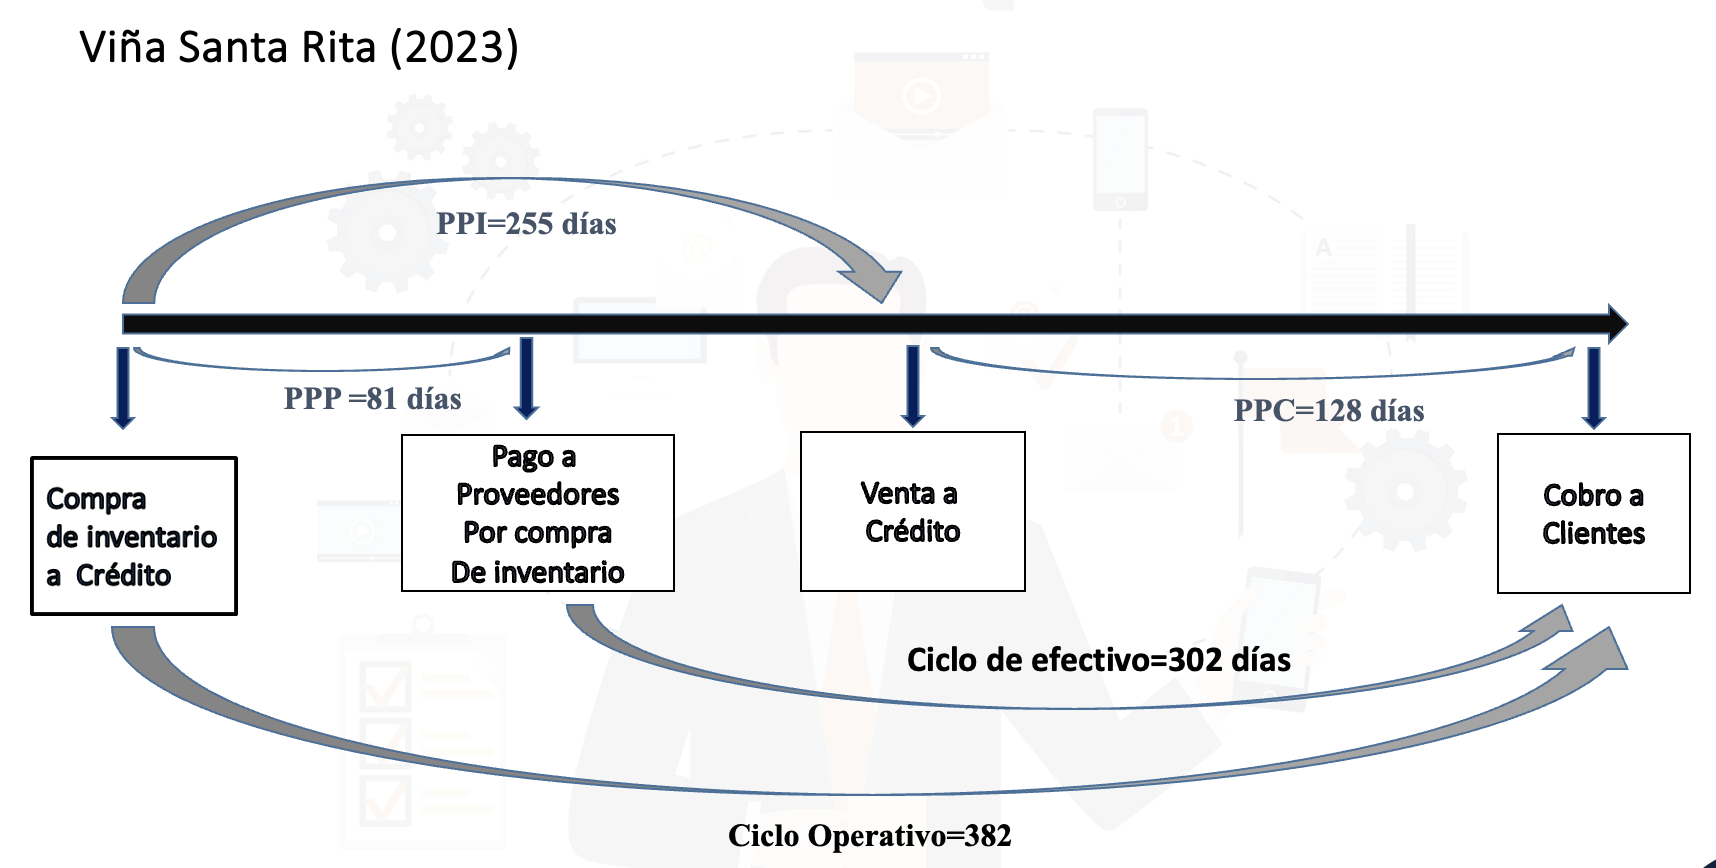
\includegraphics{Ejemplo_Sta_Rita.png}

}

\caption{Ciclo Operativo}

\end{figure}%

\begin{center}\rule{0.5\linewidth}{0.5pt}\end{center}

\begin{itemize}
\tightlist
\item
  En una situación general, la empresa tiene dos opciones de
  financiamiento de corto plazo:

  \begin{itemize}
  \tightlist
  \item
    \begin{enumerate}
    \def\labelenumi{\arabic{enumi}.}
    \tightlist
    \item
      Usar financiamiento de corto plazo, tales como factoring, línea
      crédito, créditos bancarios etc., lo cual genera un costo
      financiero por la tasa de interés y otros de la deuda financiera.
    \end{enumerate}
  \item
    \begin{enumerate}
    \def\labelenumi{\arabic{enumi}.}
    \setcounter{enumi}{1}
    \tightlist
    \item
      Si tuviera excedentes de Capital de Trabajo, tiene un costo de
      oportunidad ya que esos recursos podrían estar invertidos en
      depósitos a plazo, fondos mutuos, etc. y se dejaría de generar
      ganancia por intereses. (ingresos financieros)
    \end{enumerate}
  \end{itemize}
\end{itemize}

\begin{center}\rule{0.5\linewidth}{0.5pt}\end{center}

\subsection{Paso 2: Cálculos en administración del Ciclo de
Efectivo}\label{paso-2-cuxe1lculos-en-administraciuxf3n-del-ciclo-de-efectivo}

\begin{itemize}
\tightlist
\item
  \begin{enumerate}
  \def\labelenumi{\arabic{enumi}.}
  \tightlist
  \item
    Calculo de POM.
  \end{enumerate}
\item
  \begin{enumerate}
  \def\labelenumi{\arabic{enumi}.}
  \setcounter{enumi}{1}
  \tightlist
  \item
    Calculo Modelo LEC: Lote Económico de Compras (Baumol)
  \end{enumerate}
\item
  \begin{enumerate}
  \def\labelenumi{\arabic{enumi}.}
  \setcounter{enumi}{2}
  \tightlist
  \item
    Miller-Orr, Saldo óptimo de efectivo, con límites y saldo para
    inversión de corto plazo en equivalentes al efectivo.
  \end{enumerate}
\end{itemize}

\begin{center}\rule{0.5\linewidth}{0.5pt}\end{center}

\subsection{1. Calculo de POM.}\label{calculo-de-pom.}

\begin{itemize}
\tightlist
\item
  Determinar la pérdida operativa mínima:
\end{itemize}

\paragraph{\texorpdfstring{1. \textbf{Rotación de
Caja}:}{1. Rotación de Caja:}}\label{rotaciuxf3n-de-caja-1}

\[
   R_c = \frac{\text{360}}{\text{Ciclo de Caja}}
   \] - \(R_c\): Rotación de caja, mide cuántas veces la empresa
``gira'' su efectivo durante el año.

\[
   R_c = \frac{360}{\text{302 dias}}  \approx 1,19
   \]

\begin{center}\rule{0.5\linewidth}{0.5pt}\end{center}

\subsection{Interpretación}\label{interpretaciuxf3n}

\begin{itemize}
\item
  Este resultado indica que la rotación de las cuentas en el período es
  de aproximadamente 1.19 veces por año.
\item
  Esto sugiere que la empresa convierte sus cuentas en efectivo
  alrededor de 1.19 veces al año, ya sea a través de inventarios o
  cuentas por cobrar, según el contexto.
\end{itemize}

\begin{center}\rule{0.5\linewidth}{0.5pt}\end{center}

\subsection{2. Calcular Caja mínima o Saldo medio de Tesorería: (Egresos
anuales/Rotación
Caja)}\label{calcular-caja-muxednima-o-saldo-medio-de-tesoreruxeda-egresos-anualesrotaciuxf3n-caja}

\begin{itemize}
\tightlist
\item
  Para calcular los egresos anuales, consideraremos las siguientes
  partidas clave del flujo de efectivo:

  \begin{enumerate}
  \def\labelenumi{\arabic{enumi}.}
  \tightlist
  \item
    \textbf{Pagos a proveedores por bienes y servicios}: Estos egresos
    representan los costos operativos esenciales para mantener el ciclo
    productivo de la empresa.
  \item
    \textbf{Pagos a y por cuenta de los empleados}: Incluye salarios,
    bonos y otros beneficios, reflejando el gasto en capital humano
    necesario para las operaciones.
  \item
    \textbf{Otros pagos por actividades de operación}: Comprende otros
    egresos menores que impactan en la caja y son parte de los costos
    operativos, como gastos administrativos o pagos menores.
  \end{enumerate}
\end{itemize}

\begin{center}\rule{0.5\linewidth}{0.5pt}\end{center}

\subsection{Calculo de Egresos
Anuales}\label{calculo-de-egresos-anuales}

\begin{itemize}
\tightlist
\item
  \textbf{Egresos Anuales:} \[
  \text{Egresos Anuales} = 125.825.795.000 + 26.234.231.000 + 8.780.316.000
  \]
\end{itemize}

\[
\text{Egresos Anuales} = 160.840.342.000
\]

\textbf{Caja Mínima:}

\[
\text{Caja Mínima} = \frac{\text{Egresos Anuales}}{\text{Rotación de Caja}} = \frac{160.840.342.000}{1,19} \approx 135.588.957.983
\]

\begin{center}\rule{0.5\linewidth}{0.5pt}\end{center}

\subsection{Interpretación de los
Cálculos}\label{interpretaciuxf3n-de-los-cuxe1lculos}

Egresos Anuales:

\begin{itemize}
\tightlist
\item
  Representan la salida total de efectivo necesaria para la operación
  anual.
\item
  Incluyen pagos esenciales como proveedores, empleados y gastos
  menores.
\end{itemize}

Caja Mínima:

\begin{itemize}
\tightlist
\item
  Muestra el efectivo mínimo para operar sin interrupciones.
\item
  Asegura liquidez para cubrir compromisos de corto plazo y enfrentar
  imprevistos.
\end{itemize}

\begin{center}\rule{0.5\linewidth}{0.5pt}\end{center}

\subsection{3. Cálculo de la Pérdida Operativa Mínima
(POM)}\label{cuxe1lculo-de-la-puxe9rdida-operativa-muxednima-pom}

\begin{itemize}
\item
  \textbf{Definición}: La POM representa la pérdida de rentabilidad
  asociada a mantener efectivo en caja, en lugar de invertirlo en
  activos alternativos.
\item
  \textbf{Cálculo}: \[
   \text{POM} = \text{Caja Mínima} \times \text{Costo de Oportunidad}
   \]
\item
  \textbf{Interpretación}:

  \begin{itemize}
  \tightlist
  \item
    La \textbf{POM} indica el monto que la empresa estaría perdiendo
    anualmente al mantener un saldo mínimo de caja.
  \item
    Destaca la importancia de equilibrar la \textbf{liquidez} con la
    \textbf{rentabilidad} mediante una gestión óptima de recursos.
  \end{itemize}
\end{itemize}

\begin{center}\rule{0.5\linewidth}{0.5pt}\end{center}

\subsection{3. Cálculo de la Pérdida Operativa Mínima
(POM)}\label{cuxe1lculo-de-la-puxe9rdida-operativa-muxednima-pom-1}

\[
\text{POM} = 135.588.957.983 \times 0,08 = 10.847.116.638,64
\]

\begin{itemize}
\tightlist
\item
  \textbf{Interpretación de la POM}:

  \begin{itemize}
  \tightlist
  \item
    La Pérdida Operativa Mínima representa el costo de mantener el
    efectivo sin invertirlo en activos que generen rentabilidad.
  \item
    Este monto indica una ``pérdida'' teórica de oportunidades de
    inversión, basada en el costo de oportunidad del capital (8\% en
    este caso).
  \item
    Es una herramienta para evaluar si el efectivo disponible podría ser
    mejor utilizado en inversiones rentables para optimizar la
    eficiencia financiera.
  \end{itemize}
\end{itemize}

\subsubsection{Referencia Costo de Oportunidad
(WACC)}\label{referencia-costo-de-oportunidad-wacc}

\begin{itemize}
\tightlist
\item
  \href{https://repositorio.uchile.cl/bitstream/handle/2250/181880/Tesis\%20-\%20Alfonso\%20Olmos\%20-\%20Parte\%20II.pdf?sequence=2}{Tesis
  - Alfonso Olmos}
\end{itemize}

\begin{center}\rule{0.5\linewidth}{0.5pt}\end{center}

\subsection{Paso 2: Cálculos en administración del Ciclo de
Efectivo}\label{paso-2-cuxe1lculos-en-administraciuxf3n-del-ciclo-de-efectivo-1}

\begin{itemize}
\tightlist
\item
  \begin{enumerate}
  \def\labelenumi{\arabic{enumi}.}
  \tightlist
  \item
    Calculo de POM.
  \end{enumerate}
\item
  \begin{enumerate}
  \def\labelenumi{\arabic{enumi}.}
  \setcounter{enumi}{1}
  \tightlist
  \item
    \textbf{Calculo Modelo LEC: Lote Económico de Compras (Baumol)}
  \end{enumerate}
\item
  \begin{enumerate}
  \def\labelenumi{\arabic{enumi}.}
  \setcounter{enumi}{2}
  \tightlist
  \item
    Miller-Orr, Saldo óptimo de efectivo, con límites y saldo para
    inversión de corto plazo en equivalentes al efectivo.
  \end{enumerate}
\end{itemize}

\begin{center}\rule{0.5\linewidth}{0.5pt}\end{center}

\subsection{Modelo LEC: Lote Económico de Compras (Modelo
Baumol)}\label{modelo-lec-lote-econuxf3mico-de-compras-modelo-baumol}

\begin{itemize}
\tightlist
\item
  \textbf{Objetivo}: Calcular el nivel óptimo de efectivo a mantener en
  caja.
\item
  Este modelo se aplica en condiciones de certeza, teniendo en cuenta:

  \begin{itemize}
  \tightlist
  \item
    Costos de transacción al convertir valores en efectivo.
  \item
    Rentabilidad de mantener el dinero invertido.
  \end{itemize}
\item
  \textbf{Dos enfoques}:

  \begin{itemize}
  \tightlist
  \item
    Hacer conversiones pequeñas y frecuentes, reduciendo la pérdida de
    rentabilidad, pero aumentando los costos de transacción.
  \item
    Hacer conversiones grandes y poco frecuentes, lo que disminuye los
    costos de transacción, pero aumenta la pérdida de rentabilidad.
  \end{itemize}
\end{itemize}

\begin{center}\rule{0.5\linewidth}{0.5pt}\end{center}

\subsection{Fórmula del Modelo LEC}\label{fuxf3rmula-del-modelo-lec}

\[
C(o) = \sqrt{\frac{2 \cdot b \cdot M}{i}}
\]

\begin{itemize}
\tightlist
\item
  \textbf{Donde}:

  \begin{itemize}
  \tightlist
  \item
    \(C(o)\): Monto óptimo de cada transacción (\$).
  \item
    \(b\): Costo de cada transacción (\$).
  \item
    \(M\): Monto total de efectivo necesario (\$).
  \item
    \(i\): Costo de oportunidad o tasa de interés.
  \end{itemize}
\end{itemize}

\begin{center}\rule{0.5\linewidth}{0.5pt}\end{center}

\subsection{Cálculo del Monto Óptimo de Efectivo de Viña Santa
Rita}\label{cuxe1lculo-del-monto-uxf3ptimo-de-efectivo-de-viuxf1a-santa-rita}

\textbf{Datos}:

\begin{itemize}
\item
  \textbf{Monto total mensual de egresos}:\\
  \[
  M = \frac{160,840,342,000}{12} \approx 13,403,361,833.33
  \]
\item
  \textbf{Costo de cada transacción}:\\
  \[
  b = 150
  \]
\item
  \textbf{Tasa de interés mensual (i)}:

  \begin{itemize}
  \tightlist
  \item
    Rentabilidad promedio del mercado financiero chileno: \(i = 0.0065\)
    (aproximadamente 0.65\% mensual)
  \end{itemize}
\end{itemize}

\begin{center}\rule{0.5\linewidth}{0.5pt}\end{center}

\subsection{Cálculo del Monto Óptimo de
Transacción}\label{cuxe1lculo-del-monto-uxf3ptimo-de-transacciuxf3n}

\[
C(o) = \sqrt{\frac{2 \cdot 150 \cdot 13.403.361.833,33}{0.0065}} = \sqrt{6.178.674.149.307,69} \approx 2.485.679,38
\]

\begin{itemize}
\tightlist
\item
  \textbf{Monto óptimo de cada transacción}: \[
  \approx 2.485.679
  \]
\end{itemize}

\begin{center}\rule{0.5\linewidth}{0.5pt}\end{center}

\subsection{Interpretación de los Resultados del Monto Óptimo de
Transacción}\label{interpretaciuxf3n-de-los-resultados-del-monto-uxf3ptimo-de-transacciuxf3n}

\begin{itemize}
\item
  El cálculo indica un \textbf{monto óptimo de efectivo} de
  aproximadamente \$2,485,679.38 por transacción.
\item
  Esto sugiere que, para minimizar costos de transacción y maximizar la
  eficiencia de caja, la empresa debería realizar transacciones de
  efectivo en este monto.
\item
  \textbf{Interpretación adicional}:

  \begin{itemize}
  \tightlist
  \item
    Un mayor número de transacciones pequeñas aumentaría los costos de
    transacción sin optimizar el rendimiento de caja.
  \item
    Transacciones grandes menos frecuentes podrían reducir estos costos
    pero aumentarían el riesgo de mantener altos montos de efectivo
    inactivo.
  \item
    Este equilibrio optimizado entre costo de transacción y costo de
    oportunidad permite mantener la liquidez con menor impacto en la
    rentabilidad.
  \end{itemize}
\end{itemize}

\begin{center}\rule{0.5\linewidth}{0.5pt}\end{center}

\subsection{Paso 2: Cálculos en administración del Ciclo de
Efectivo}\label{paso-2-cuxe1lculos-en-administraciuxf3n-del-ciclo-de-efectivo-2}

\begin{itemize}
\tightlist
\item
  \begin{enumerate}
  \def\labelenumi{\arabic{enumi}.}
  \tightlist
  \item
    Calculo de POM.
  \end{enumerate}
\item
  \begin{enumerate}
  \def\labelenumi{\arabic{enumi}.}
  \setcounter{enumi}{1}
  \tightlist
  \item
    Calculo Modelo LEC: Lote Económico de Compras (Baumol)
  \end{enumerate}
\item
  \begin{enumerate}
  \def\labelenumi{\arabic{enumi}.}
  \setcounter{enumi}{2}
  \tightlist
  \item
    \textbf{Miller-Orr, Saldo óptimo de efectivo, con límites y saldo
    para inversión de corto plazo en equivalentes al efectivo.}
  \end{enumerate}
\end{itemize}

\begin{center}\rule{0.5\linewidth}{0.5pt}\end{center}

\subsection{Recalculando el Modelo de Miller y Orr en
Pesos}\label{recalculando-el-modelo-de-miller-y-orr-en-pesos}

\subsubsection{Ajuste del Saldo Mínimo de Caja
Diario}\label{ajuste-del-saldo-muxednimo-de-caja-diario}

Para reflejar el \textbf{saldo mínimo de caja diario}, dividimos el
saldo anual por 360:

\[
L_{\text{diario}} = \frac{135.588.957.983}{360} \approx 376.636.050
\]

\begin{itemize}
\tightlist
\item
  \textbf{Saldo mínimo de caja diario (L)}: \$376.636.050
\end{itemize}

\begin{center}\rule{0.5\linewidth}{0.5pt}\end{center}

\subsubsection{Parámetros del Modelo en
Pesos}\label{paruxe1metros-del-modelo-en-pesos}

\begin{itemize}
\tightlist
\item
  \textbf{Saldo mínimo de caja diario (L)}: \$376.636.050
\item
  \textbf{Costo de transacción (b)}: \$150
\item
  \textbf{Varianza de los flujos diarios de efectivo ((\sigma\^{}2))}:
  \$1.500.000
\item
  \textbf{Tasa de interés diaria (i)}: 0,00021
\end{itemize}

\begin{center}\rule{0.5\linewidth}{0.5pt}\end{center}

\subsubsection{Aplicando la Fórmula de Miller y
Orr}\label{aplicando-la-fuxf3rmula-de-miller-y-orr}

La fórmula para calcular el \textbf{saldo óptimo de efectivo (Z)} es:

\[
Z = L + \sqrt[3]{\dfrac{3b\sigma^2}{4i}}
\]

\begin{center}\rule{0.5\linewidth}{0.5pt}\end{center}

\subsubsection{Cálculo Paso a Paso}\label{cuxe1lculo-paso-a-paso}

\paragraph{1. Calcular el Numerador}\label{calcular-el-numerador}

\[
\text{Numerador} = 3 \times b \times \sigma^2 = 3 \times 150 \times 1.500.000 = 675.000.000
\]

\paragraph{2. Calcular el Denominador}\label{calcular-el-denominador}

\[
\text{Denominador} = 4 \times i = 4 \times 0,00021 = 0,00084
\]

\paragraph{3. Calcular la Fracción}\label{calcular-la-fracciuxf3n}

\[
\frac{\text{Numerador}}{\text{Denominador}} = \frac{675.000.000}{0,00084} = 803.571.428.571,43
\]

\begin{center}\rule{0.5\linewidth}{0.5pt}\end{center}

\paragraph{4. Calcular la Raíz
Cúbica}\label{calcular-la-rauxedz-cuxfabica}

\[
\sqrt[3]{803.571.428.571,43} \approx 9.283
\]

\paragraph{5. Calcular el Saldo Óptimo
(Z)}\label{calcular-el-saldo-uxf3ptimo-z}

\[
Z = L + \sqrt[3]{\dfrac{3b\sigma^2}{4i}} = 376.636.050 + 9.283 = 376.645.333
\]

\begin{center}\rule{0.5\linewidth}{0.5pt}\end{center}

\subsubsection{Determinación de los
Límites}\label{determinaciuxf3n-de-los-luxedmites}

\paragraph{Límite Superior (H)}\label{luxedmite-superior-h}

\[
\begin{align*}
H &= 3Z - 2L \\
  &= 3 \times 376.645.333 - 2 \times 376.636.050 \\
  &= 1.129.935.999 - 753.272.100 \\
  &= 376.663.899
\end{align*}
\]

\paragraph{Límite Inferior (L)}\label{luxedmite-inferior-l}

\[
L = 376.636.050
\]

\begin{center}\rule{0.5\linewidth}{0.5pt}\end{center}

\subsection{Resultados Finales en
Pesos}\label{resultados-finales-en-pesos}

\begin{itemize}
\tightlist
\item
  \textbf{Saldo mínimo de caja diario (L)}: \$376.636.050
\item
  \textbf{Saldo óptimo de efectivo (Z)}: \$376.645.333
\item
  \textbf{Límite superior (H)}: \$376.663.899
\end{itemize}

\begin{center}\rule{0.5\linewidth}{0.5pt}\end{center}

\subsection{Interpretación de los
Resultados}\label{interpretaciuxf3n-de-los-resultados}

\subsubsection{Saldo Mínimo de Caja Diario
(L)}\label{saldo-muxednimo-de-caja-diario-l}

\begin{itemize}
\tightlist
\item
  \textbf{\$376.636.050} es el saldo mínimo que la empresa debe mantener
  diariamente para asegurar sus operaciones sin problemas de liquidez.
\end{itemize}

\subsubsection{Saldo Óptimo de Efectivo
(Z)}\label{saldo-uxf3ptimo-de-efectivo-z}

\begin{itemize}
\tightlist
\item
  \textbf{\$376.645.333} es el saldo óptimo que equilibra los costos de
  mantener efectivo y los costos de transacción.
\end{itemize}

\begin{center}\rule{0.5\linewidth}{0.5pt}\end{center}

\subsubsection{Límite Superior (H)}\label{luxedmite-superior-h-1}

\begin{itemize}
\tightlist
\item
  \textbf{\$376.663.899} es el límite superior. Al alcanzarlo, la
  empresa debe invertir el excedente para evitar fondos ociosos.
\end{itemize}

\subsubsection{Operaciones Diarias}\label{operaciones-diarias}

\begin{itemize}
\tightlist
\item
  \textbf{Si el saldo cae por debajo de L}: Convertir inversiones en
  efectivo hasta alcanzar Z.
\item
  \textbf{Si el saldo supera H}: Invertir el excedente hasta reducir el
  saldo a Z.
\end{itemize}

\begin{center}\rule{0.5\linewidth}{0.5pt}\end{center}

\subsection{Conclusiones}\label{conclusiones}

\begin{itemize}
\tightlist
\item
  \textbf{Ajuste en Pesos}: Al realizar los cálculos en pesos, obtenemos
  resultados más precisos y relevantes para la gestión financiera.
\item
  \textbf{Aplicación del Modelo}: El modelo de Miller y Orr ayuda a
  mantener un equilibrio óptimo entre liquidez y rentabilidad.
\item
  \textbf{Margen Estrecho}: La diferencia reducida entre los límites
  indica una alta estabilidad en los flujos de efectivo.
\end{itemize}

\begin{center}\rule{0.5\linewidth}{0.5pt}\end{center}

\subsection{Recomendaciones}\label{recomendaciones}

\begin{enumerate}
\def\labelenumi{\arabic{enumi}.}
\tightlist
\item
  \textbf{Monitoreo Diario}: Implementar sistemas para seguimiento
  diario del saldo de caja en pesos.
\item
  \textbf{Actualizar Parámetros}:

  \begin{itemize}
  \tightlist
  \item
    Revisar periódicamente la \textbf{varianza ((\sigma\^{}2))} de los
    flujos de efectivo.
  \item
    Actualizar la \textbf{tasa de interés (i)} según el mercado.
  \end{itemize}
\item
  \textbf{Análisis de Sensibilidad}: Evaluar cómo cambios en los
  parámetros afectan el modelo.
\end{enumerate}

\begin{center}\rule{0.5\linewidth}{0.5pt}\end{center}

\subsection{Referencias}\label{referencias-1}

\begin{itemize}
\tightlist
\item
  \textbf{Modelo de Miller y Orr}:

  \begin{itemize}
  \tightlist
  \item
    Miller, M. H., \& Orr, D. (1966). \emph{A Model of the Demand for
    Money by Firms}.
  \end{itemize}
\item
  \textbf{Datos Financieros}:

  \begin{itemize}
  \tightlist
  \item
    Estados financieros de Viña Santa Rita.
  \end{itemize}
\item
  \textbf{Tasa de Interés}:

  \begin{itemize}
  \tightlist
  \item
    Rentabilidad promedio del mercado financiero chileno.
  \end{itemize}
\end{itemize}

\begin{center}\rule{0.5\linewidth}{0.5pt}\end{center}




\end{document}
